\documentclass[11pt]{article}

\usepackage[backend=bibtex]{biblatex}
\usepackage[utf8]{inputenc}
\usepackage{amsmath}
\usepackage{amssymb}
\usepackage{anysize}
\usepackage{graphicx}
\graphicspath{ {../../images/} }
\usepackage{color}
\usepackage{xcolor}
\usepackage{algorithm2e}
\usepackage{pgfplots}
\usepackage{hyperref}
\usepackage{booktabs}

\usepackage{graphicx}
\usepackage{caption}
\usepackage{subcaption}

\bibliography{bibliography.bib}

\usepackage{tikz}
\usetikzlibrary{shapes,arrows}

\definecolor{mygreen}{rgb}{0,0.6,0}
\definecolor{mygray}{rgb}{0.5,0.5,0.5}
\definecolor{mypurple}{rgb}{0.58,0,0.82}

\usepackage{listings}

\usepackage{caption}
\DeclareCaptionFont{white}{\color{white}}
\DeclareCaptionFormat{listing}{\colorbox{gray}{\parbox[c]{\textwidth}{#1#2#3}}}

\setlength\parindent{0pt}
\setlength{\parskip}{10pt}

\marginsize{2cm}{2cm}{1cm}{1cm}

\usepackage{titlesec}
\titleformat{\section}{\large\bfseries}{\thesection}{1em}{}

\begin{document}

%  Title and authors
   \begin{center}
     {\huge\bfseries B31XP Robotics project\\ Robotic object follower}\\
      \vspace{2ex}
      \textsc{Andrey Pak, Donatas Kozlovskis, Enric Cornellà,\\ Fernando Garcia,  Igor Peric}
   \end{center}
   \vspace{2ex}%

%  Abstract
\begin{abstract}
This project presents a small, easy to build low-cost robot system, that is able to find coloured signs on the floor and implement the associated actions, e.g. stop, turn, pause, etc.
The robot hardware uses Raspberry Pi to control a set of motors, sensors and servo actuators. 
Report provides information about done review the hardware design and implementation of software using open source tools as C++ and OpenCV libraries. 
\end{abstract}
 
%%%%%%%%%%%%%%%%%%%%%%%%%%%%%
\section{Software}


Conceptual overview of software architecture and its parts is given on figure \ref{fig:soft_overview}. All components will be discussed and described in detail in this section of the report. 

%\begin{figure}[th!]
%\center
%\includegraphics[scale=0.7]{images/software-architecture.png}
%\caption{Overview of software architecture of the solution}
%\end{figure}


\begin{figure}[!ht]
	\hspace{-1cm}
	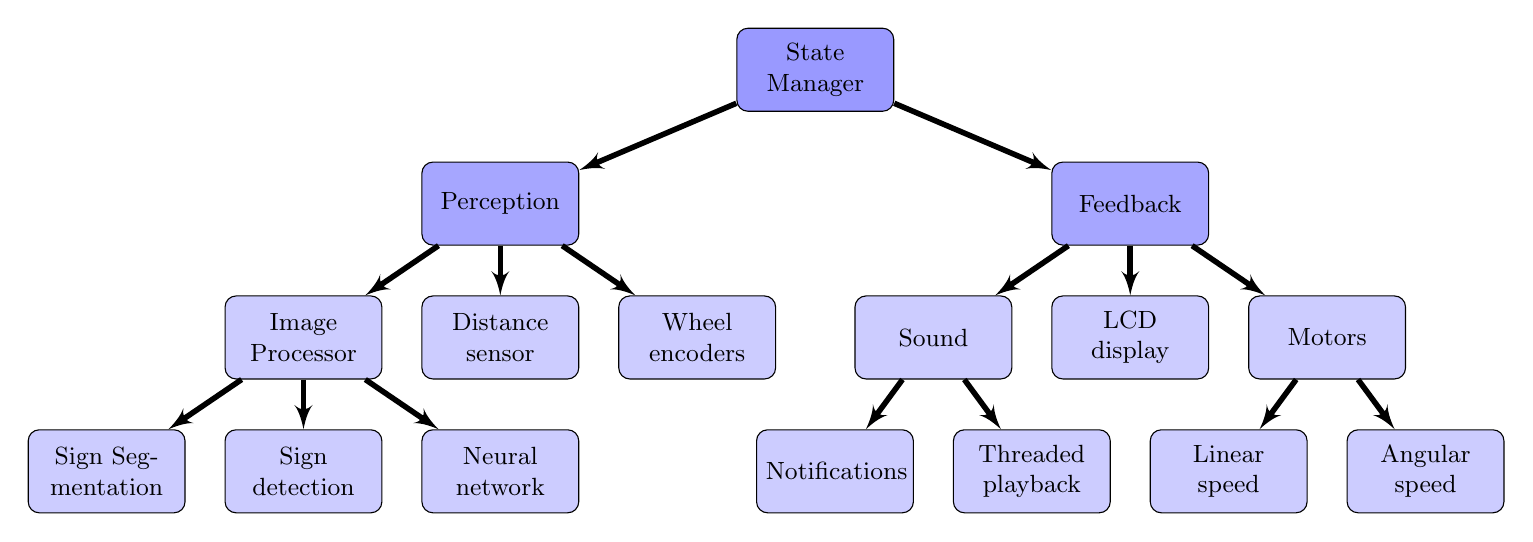
\begin{tikzpicture}[node distance = 2.5cm, auto]
	% % % % % % % % % % % % % % % % % % % % % % % % % % % % % %
	% Define styles
	\tikzstyle{block} = [rectangle, draw, fill=blue!20, text width=5em, text centered, 
					     rounded corners, minimum height=3em, font=\small]
	\tikzstyle{line} = [draw, -latex', line width =2pt]
	
	% % % % % % % % % % % % % % % % % % % % % % % % % % % % % %
	% Place nodes
	% parent
	\node [block,  fill=blue!40] (sm) {State Manager};
	% child level 1
	\node [block, fill=blue!35, below of=sm, node distance = 1.7 cm, xshift=-4.cm] (pc) {Perception};
	\node [block, fill=blue!35, below of=sm, node distance = 1.7 cm, xshift=4.cm] (fb) {Feedback};
	% child level 2 left
	\node [block, below of=pc, node distance = 1.7cm] (ds) {Distance sensor};
	\node [block, left of=ds] (ip) {Image Processor};
	\node [block, right of=ds,  node distance = 2.5 cm] (we) {Wheel encoders};
	% %third level left
	\node [block, below of=ip, node distance = 1.7 cm] (sgd) {Sign detection};
	\node [block, left of=sgd] (sgm) {Sign Segmentation};
	\node [block, right of=sgd] (nn) {Neural network};
	
	% child level 2 right
	\node [block, below of=fb, node distance = 1.7 cm] 						(ld) {LCD display};
	\node [block, left of=ld] 	(sn) {Sound};
	\node [block, right of=ld] (mt) {Motors};
	
	% %third level right
	\node [block, below of=sn, node distance = 1.7 cm, xshift=-1.25cm] (ntf) {Notifications};
	\node [block, below of=sn, node distance = 1.7 cm, xshift=1.25cm] (thr) {Threaded playback};
	% %third level right
	\node [block, below of=mt, node distance = 1.7 cm, xshift=-1.25cm] (lns) {Linear speed};
	\node [block, below of=mt, node distance = 1.7 cm, xshift=1.25cm] (ags) {Angular speed};
	
%	\node [block, right of=left,  node distance = 3 cm] (right) {Turn right};
	% Draw edges
	\path [line] (sm) -- (fb);
	\path [line] (sm) -- (pc);
	% %
	\path [line] (pc) -- (ip);
	\path [line] (pc) -- (we);
	\path [line] (pc) -- (ds);
	% %
	\path [line] (fb) -- (sn);
	\path [line] (fb) -- (mt);
	\path [line] (fb) -- (ld);
	% %  third level image proc
	\path [line] (ip) -- (sgm);
	\path [line] (ip) -- (sgd);
	\path [line] (ip) -- (nn);
	% %  third level sound
	\path [line] (sn) -- (ntf);
	\path [line] (sn) -- (thr);
	% %  third level motors
	\path [line] (mt) -- (lns);
	\path [line] (mt) -- (ags);
	\end{tikzpicture}
	\caption{Overview of software architecture of the solution}
	\label{fig:soft_overview}
\end{figure}



\section{State machine}


One of the most common and intuitive approaches for implementation of software controller for hardware system is state-machine approach. It is fairly simple concept, with only a couple of important considerations.

System controlled by state machine has certain number of possible, unique and well defined states that it can be in at every moment of execution. State defines the behaviour of the system in every discrete moment of time, including three important aspects: sensor data acquisition, output behaviour computation and state transition check. In other words, every state has it is own logic for doing all of these three mentioned steps, which gives a lot of variability for possible control scenarios. It is worth mentioning that some states might skip certain steps or perform some steps more than once without state transition check, for example.

\paragraph{System states}

At any moment of time robot can be in one of the following state seen in figure \ref{fig:algorithm-diagram}.

\begin{figure}[ht!]
	\centering
	\includegraphics[width=0.7\textwidth]{newDiagram.png}
	\caption{State transition algorithm}
	\label{fig:algorithm-diagram}
\end{figure}

\textit{IDLE} state sets both angular and linear speed to zero and waits for any of the segmented object currently inside view to go away, after which it goes to WIGGLING state.

\textit{WIGGLING} state rotates the robot around its vertical axis with constant angular and zero linear speed until a sign is detected. After detecting a sign it switches to APPROACHING\_SIGN state.

\textit{APPROACHING\_SIGN} state moves the robot close to the sign it has seen in the previous state. It does this by setting the linear speed to constant value and adjusting angular speed all the time based on the horizontal position of the target sign in the view. Robot will move in the direction needed to align the sign to the center of the screen, and it will do that proportionally to the distance of the target to the center.

\textit{EXECUTING\_COMMAND} state has different behavior depending on the type of the sign that was seen in the state before. If it was goal sign, it will switch to the GAME\_OVER state and the game will end. If it was stop sign, robot will just wait for certain predefined time-out (5 seconds) and switch to state MARCHING\_FORWARD. If it was the arrow sign, robot will turn desired angle and switch switch to state MARCHING\_FORWARD.

\textit{MARCHING\_FORWARD} state sets the linear speed to constant and angular to zero. In this state robot constantly monitors camera image stream and can potentially switch to APPROACHING\_SIGN state once a sign is detected in perceptive area of the image.

\textit{GAME\_OVER} state is entered after goal sign is approached. After displacing notification about game completion (through audio and visual feedback), robot remains idle until hardware button is pressed for the start of the new game.

%\begin{figure}[th!]
%	\centering
%	\includegraphics[scale=1]{algorithm-diagram.png}
%	\caption{State transition algorithm}
%	\label{fig:algorithm-diagram}
%\end{figure}

%\paragraph{Sensor data acquisition}

First step in state machine control loop is sensor acquisition step. If possible, data is acquired from all input sensors in order to determine current state of the environment. This includes acquisition of camera image using OpenCV, reading heading angle from motor driver and reading distances from ultrasonic sensor driver.

Last values of all the readings are always stored in local members of the class, so they can be referenced between successive acquisitions.

%\paragraph{Output behavior computation}

Based on the sensed input data values for all output units are being calculated. This includes linear and angular wheel velocities, message for LCD display, sound to be played on speakers, etc.

%\paragraph{State transition condition}

Every state has to have clearly defined condition which will make the system switch to any of the other states. System remains in the current state until one of the state transition conditions has been met.





%%%%%%%%%%%%%%%%%%%%%%%%%%%%%
\section{Vision module}


The task of vision subsystem is to handle the image data acquired from Raspbery Pi camera. This handling includes two basic subtasks: sign detection and sign recognition.

Three basic signs detected and recognized by the system are shown on figure below.

-----------(color images of all three signs taken by camera)

Different methods and challenges encountered in vision module are described and discussed separately in the following chapters of the report.

\subsubsection{Thresholding}

The first and the most intuitive approach to sign detection procedure was simple color thresholding, since signs which had to be detected are purely red.

The initial choice for color thresholding was HSV color space. Ranges of H (hue), S (saturation) and V (value) channels are [0,180], [0, 255] and [0, 255], respectively. In order to segment only red color, values of H (hue) channel greater than 170 and lower than 10 were used, since this range represents the band of red color. Additionally, too dark (V $ < $ 40), to bright (V $ > $ 220) and non-saturated pixels (S $ < $ 40) were rejected to improve the quality of segmentation. Results are shown on the figure ~\ref{fig:color-spaces}.

\begin{figure}[th!]
	\centering
	\begin{subfigure}[b]{0.3\textwidth}
		\centering
	\includegraphics[scale=0.33]{thresholding-raw.png}
	\subcaption{Raw camera input}
	\end{subfigure}
	\begin{subfigure}[b]{0.3\textwidth}
		\centering
		\includegraphics[scale=0.7]{thresholding-hsv.png}
		\subcaption{HSV color space}
	\end{subfigure}
	\begin{subfigure}[b]{0.3\textwidth}
		\centering
		\includegraphics[scale=0.7]{thresholding-YCrCb.png}
		\subcaption{YCrCb color space}
	\end{subfigure}
	\caption{Comparison of color spaces used for thresholding}
	\label{fig:color-spaces}
\end{figure}

After some testing, YCrCb color space proved to give better results for segmentation, as shown on figure above. As a result, YCrCb color space was used in final implementation.

Usage of IR camera did not affect the recognition quality of the thresholding procedure in regular, normal lighting conditions. On the other hand, it drastically increased the accuracy in low lighting conditions, which is described in Hardware section of the report.

The biggest connected component (blob) int he thresholded image is considered to be a sign. Bounding box of the biggest blob determined the area of the thresholded image to be passed in as an input to the sign classification module. 

\subsection{Classification of the signs using statistical moments}

Taking into consideration the relatively low computational power of the hardware platform used to develop the system, priority for the chosen sign classification algorithm was low complexity.

After some thorough analysis of the available option, statistical moments proven to be the best option.

For an arbitrary binary (i.e. thresholded) input image system can compute statistical moments of desired order. The moment of importance in case of sign classification was center of mass or first order moment. It can be thought of average coordinate of all white pixels for both axes.

\begin{figure}[th!]
	\centering
	\begin{subfigure}[b]{0.25\textwidth}
		\centering
		\includegraphics[scale=0.55]{moments-arrow-raw.png}
		\subcaption{Raw camera input}
	\end{subfigure}
	\begin{subfigure}[b]{0.25\textwidth}
		\centering
		\includegraphics[scale=0.8]{moments-arrow-segm.png}
		\subcaption{Arrow}
	\end{subfigure}
	\begin{subfigure}[b]{0.2\textwidth}
		\centering
		\includegraphics[scale=0.8]{moments-cross-segm.png}
		\subcaption{Cross}
	\end{subfigure}
	\begin{subfigure}[b]{0.2\textwidth}
		\centering
		\includegraphics[scale=0.9]{moments-circle-segm.png}
		\subcaption{Circle}
	\end{subfigure}
	\caption{Visual cues for sign classification using statistical moments}
	\label{fig:statistical-moments}
\end{figure}

Figure \ref{fig:statistical-moments} demonstrates intuition behind visual cues used for discrimination of three different types of signs. By computing the distance of center of the mass (green rectangle) and center of the cropped image segment where the sign was detected (blue rectangle) we can perform initial discrimination between \textbf{arrow} and \textbf{rest two signs}. Distance is going to be close to zero in case of cross and circle since object are symmetrical around two mutually normal axes. Arrow is not symmetrical around one axis, so it's center of the mass will be slightly shifter towards the tip of the arrow and this is the property used to distinguish an arrow from the circle and cross.
Table \ref{tab:moments} shows average distance of center of the mass from image center proportional to cropped image size. Clear observation is that thresholding this distance to 10 $\%$ can give is pretty good estimate of probability that sign belongs to arrow class.

If this distance is close to zero, additional step is needed to determine is the observed sign cross or circle. Approach used in this step was investigation of zero-order moment, which gives the number of white pixels in the image. By taking the ratio of zero order moment and total number of pixels of sign area, we can distinguish between cross and circle. Intuition behind this metric lies in the fact that circle has bigger surface than cross of the same bounding box size, so the percentage of space it occupies in the cropped image area where the sign is going to be larger than if it was cross. Table \ref{tab:moments} gives suitable value of threshold of 70 $\%$.

\begin{table}[th!]
\centering
\begin{tabular}{l*{2}{c}r}
	Sign class			& Distance of first moment & Ratio of second order moment  \\
	\hline
	Arrow 				& 18.41 & 56.44  \\
	Cross            	& 1.39 & 54.20  \\
	Circle           	& 0.97 & 89.63  \\
\end{tabular}
\caption{Numerical values of statistical moments given in $\%$ wrt. image size}
\label{tab:moments}
\end{table}

Images of all three signs with drawn moments and numerical explanation of distinction between those three

\subsection{Neural network classifier}

Justification of usage neural networks.

Very brief theoretical background.

Description of the way how we train it on images (raw pixel values, segmentation pixels, hu-moments as inputs, etc)

Description of tested recognition method (sliding window, random, ...)

Performance comparison with previous method.

\subsection{Arrow angle calculation}

After sign has been classified as arrow, additional step needs to be performed in order to extract the arrow angle relative to the orientation of the robot at the moment of observation.

Description of the initial way (using moments) and failing scenarios. 

Idea of using line fitting, with slight theoretical background and results.

\subsection{Solving partial occlusion and re-detection}

Explanation of problem of partial occlusion and re-detection, when does it happen and why we want to handle it.

Explanation of perceptive area and proximity area.





\section{Further improvements}


\subsection{Robustness of sign classification}

Current sign classification approach is computationally inexpensive and has simple implementation and execution. Price paid for these benefits is low robustness, meaning that there are times when robot detects some other red object's shape as one of the three signs that it needs to classify.

In order to avoid these issues a more robust classifier is needed. Approach using artificial neural networks, Support Vector Machines or any other machine learning technique would require training classifiers on another (more powerful) CPU and loading trained classifier to the robot just for the purposes of classification.

\subsection{Complex game rules and sign diversity}

Current rules for interaction with robot rely only on couple of simple actions and available signs. Software control architecture is built in a way modular way, which enables easy addition of the new signs under assumption of robust classifier able to distinguish between all currently known signs and newly added one.

Expanding set of available signs could enrich the game experience by introducing new objectives, goals and obstacles for the children to play with.

\subsection{Hardware improvements}

Although system is currently able to perform all desired tasks, a \textit{more powerful processing hardware would make it faster, more responsive} and, thus, more fun for children to play with. Having only 6 FPS from camera limits the maximum velocity of robot movement as well, so games would look more dynamic if robot was able to move faster. 

It would, also, enable usage of more advanced and, at the same time, more robust algorithms for image processing. This would \textit{remove some limitations and conditions} put on the usage of the robot, like camera pointing only towards ground (floor) plane, maximum distance of sign placement, sign shape and color restrictions, etc.

\textit{More sensors} would enrich engagement of the children as well by providing diverse set of ways to interact with the robot. 




\clearpage


\end{document}